\chapter{Adding Battery Awareness in EASY Backfilling}
\label{cha:heuristic}

\minitoc

\section{Heuristic}

This section presents the heuristic applied in ODM to deal with its different responsibilities. We named this heuristic \emph{\systemName}. This heuristic acts in three different moments. First, Section \ref{sec:model_predictions} explains the predictions used through the \emph{\systemName}'s decisions. These predictions are made at the beginning of the time window, just one time. Then, Section \ref{sec:model_easy} describes the modifications in the EASY Backfilling heuristic to introduce battery awareness. The modified EASY Backfilling acts every time a job finishes, arrives, or new servers are available. Finally, Section \ref{sec:model_compensations} defines the compensation policies. \emph{\systemName} compensates every time step.

\subsection{Predictions}
\label{sec:model_predictions}

As presented in Section \ref{sec:offline_plan}, ODM receives two predictions from offline modules: power production and power demand. Since ODM works online, it will not predict itself but use the predictions from offline. So, this section will not focus on the forecasting method but on using its results.

\begin{figure}[!htb]
    \centering
    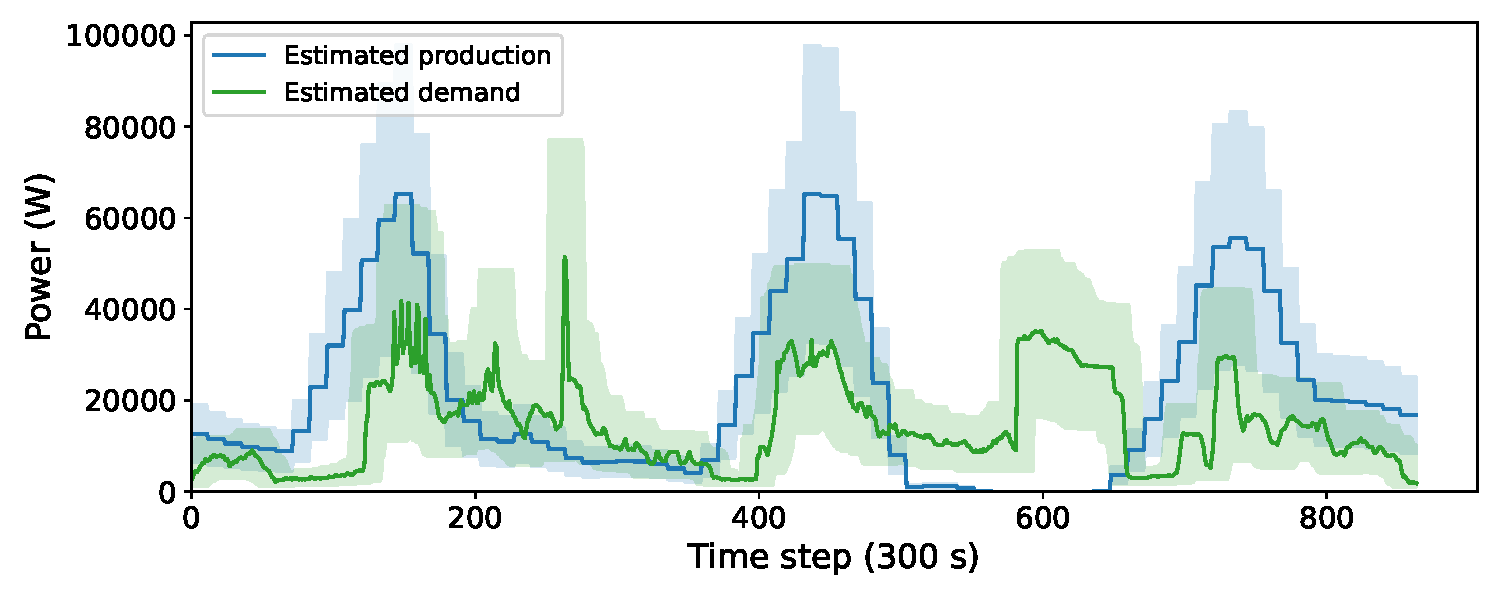
\includegraphics[scale=0.5]{Images/Heuristics/predictions.pdf}
    \caption{Renewable production and demand prediction. The blue (production) and green (demand) areas are the uncertainty given by the forecast.}
    \label{fig:predictions}
\end{figure}

Figure \ref{fig:predictions} illustrates both forecasts showing the area of uncertainty. The real value can be any value inside the uncertainty area. \emph{\systemName} uses these predictions to create different possible states of charge using equations \ref{equ:battery_state_of_charge} and \ref{equ:battery_energy}. To do so, we estimated $P_{dch}$ and $P_{ch}$ using Equations \ref{equ:battery_charge}, and \ref{equ:battery_discharge}: 
\begin{equation}
    \label{equ:battery_charge}
    P_{ch}(t) = 
    \begin{cases}
        P_{renew}^{est} - P_{load}^{est},& \text{if } P_{renew}^{est} > P_{load}^{est} \\
        0,              & \text{otherwise}
    \end{cases}
\end{equation}
\begin{equation}
    \label{equ:battery_discharge}
    P_{dch}(t) = 
    \begin{cases}
        P_{load}^{est} - P_{renew}^{est},& \text{if } P_{renew}^{est} < P_{load}^{est} \\
        0,              & \text{otherwise}
    \end{cases}
\end{equation}

Where:
\begin{itemize}
    \item \(P_{renew}^{est}\): Estimated power production from renewable;
    \item \(P_{load}^{est}\): Estimated power demanded.
\end{itemize}

Figure \ref{fig:estimated_state_of_charge} demonstrates the result of applying Equation \ref{equ:battery_state_of_charge} using nine different predictions. \emph{\systemName} calculates these SoC combining lower, median, and upper boundaries from the area presented in Figure \ref{fig:predictions} (e.g., demand lower boundary + production lower boundary, demand median + production lower boundary, demand median + production higher boundary, etc...). It is possible to notice that the state of charge can vary a lot. Section \ref{sec:model_compensations} will describe how we use these SoCs to compensate. Figure \ref{fig:estimated_state_of_charge} also illustrates both SoC upper and lower thresholds (red dashed lines). Setting upper and lower thresholds helps to increase the battery lifetime \cite{xu2016modeling}. The narrower the range, the longer the expected lifetime \cite{xu2016modeling}. However, selecting a narrow range limits the battery benefits. The figure presents both thresholds as 90-20\%, but they are parameterizable. Finally, \emph{\systemName} estimates dangerous areas in the time window. Figure \ref{fig:estimated_state_of_charge} indicates this moment. It considers a dangerous area when more than half of the predicted SoC curves are below the lower threshold. Taking Figure \ref{fig:estimated_state_of_charge} example with nine predictions, \emph{\systemName} considers the dangerous point where five curves are below 20\%. Section \ref{sec:model_easy} will explain how it uses these moments to make better scheduling decisions.

\begin{figure}[!htb]
    \centering
    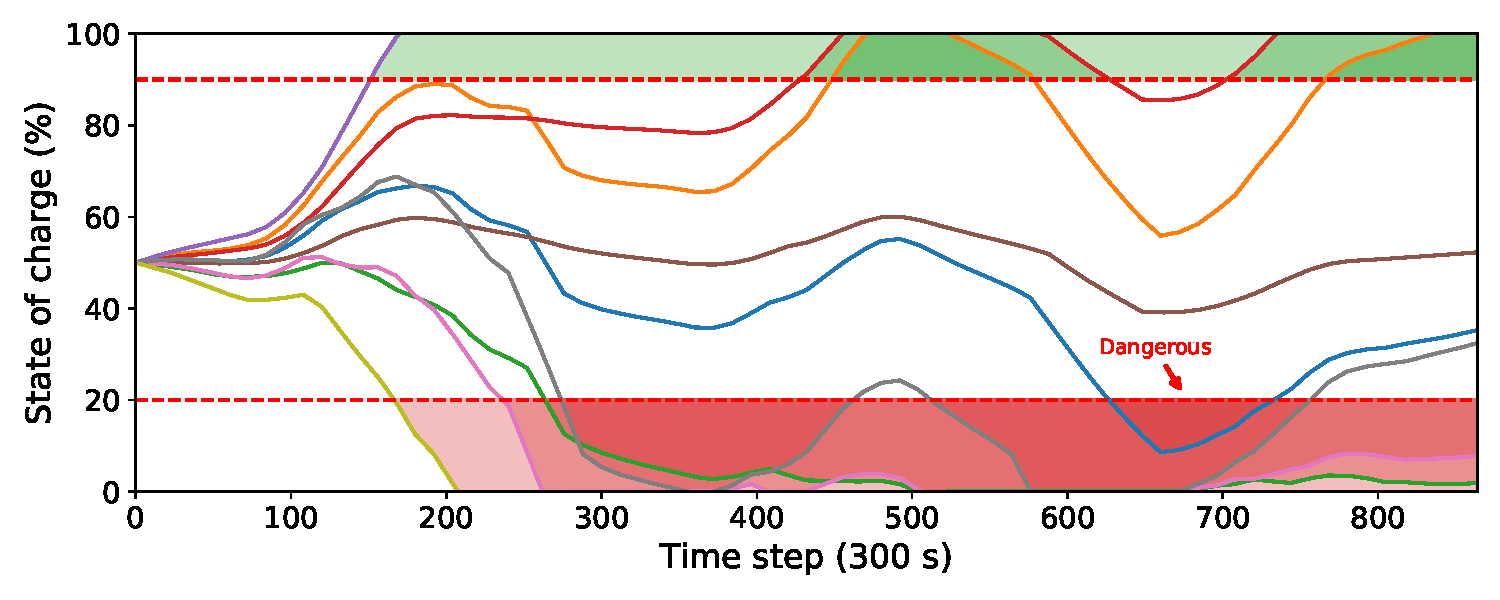
\includegraphics[scale=0.5]{Images/Heuristics/state_of_charge.pdf}
    \caption{Result of the Equation \ref{equ:battery_state_of_charge} for different predictions. The dangerous area is when 5 or more curves (so, more than half of them) are below 20\%.}
    \label{fig:estimated_state_of_charge}
\end{figure}

\subsection{Job Scheduling}
\label{sec:model_easy}

One of the most important ODM's duties is placing jobs on servers. To do so, \emph{\systemName} implements a well-known heuristic name EASY backfilling, but using two different sorts \cite{mu2001utilization, lelong2018tuning}. We detail how we use both sorts in this section. Algorithm \ref{alg:algo_scheduling_heuristic} presents the main idea. This algorithm is similar to Algorithm \ref{alg:algo_scheduling}, but with some modifications. \emph{\systemName} runs this algorithm when a job arrives, a job finishes, or there are new servers available. First, this heuristic sorts the jobs in the queue in a priority order $P_{R}$ (line 2). Then, it finds the servers to run this job (line 5). The server must be available at least at the actual time step to be chosen. Line 6 has the first modification. Usually, EASY backfilling only verifies if the servers $S$ are available now. We added the following verifications:

\begin{enumerate}
    \item It verifies if the servers $S$ are available during the entire execution, considering the walltime given by the user as the execution time. If so, it returns true. If not, it goes to the next verification;
    \item It verifies if it is possible to change the plan to keep the servers S running the entire execution. To do so, it does the following steps:
    \begin{enumerate}
        \item First, it calculates how much energy is needed. To do so, it calculates $Ed_t^{'}$ for each time step $t$ that the server sleeps, putting the server in the same state/speed as the previous time step ($t-1$). The total energy demanded is $\sum Ed_t^{'} - Ed_t$ considering all the time steps that the job executes;
        \item Then, it calculates how much energy is possible to take from future steps, putting idle servers to sleep. Let it be $E_{poss}$. Since we have to maintain the state of charge between both thresholds, we can not "migrate" all the energy to use now. So, it only considers the idle servers from the actual time step until the time step where the SoC will be equal or lower to the lower threshold. We can migrate the energy freely between the actual time step and this future one. Figure \ref{fig:idle_machines_verification} illustrates this verification;
        \item Then, it tests if $E_{poss} >= \sum Ed_t^{'} - Ed_t$. If this is false, it returns false and does not change the plan. If this is true, it makes $Ed_t = Ed_t^{'}$, changes the server speeds, and recalculates the planned state of charge (using Equation \ref{equ:battery_state_of_charge}).
    \end{enumerate}
\end{enumerate}

\IncMargin{1em}
\begin{algorithm}[!htb]
    \LinesNumbered
    \footnotesize
    \SetAlgoLined
    \SetKwInOut{Input}{input}\SetKwInOut{Output}{output}
    \Input{Queue $Q$ of waiting jobs, $P_{R}$ as priority order, and $P_{B}$ as backfilling order.}
    \Output{None (calls to \textit{Start()})}
    \Begin{
        Sort $Q$ according to $P_{R}$\;
        \For{job $j$ in $Q$}{
            Pop $j$ from $Q$\;
            $S \leftarrow$ \textit{select\_servers($j$)}\;
            \uIf{$j$ can be started and finished in servers $S$}{
                \textit{Start($j$, $S$)}\;
            }\Else{
                Reserve $j$ at the earliest time possible according to the walltime of the currently running jobs\;
                Sort $Q$ according to $P_{B}$\;
                \For{job $j^{'}$ in $Q$}{
                    $S \leftarrow$ \textit{select\_servers($j^{'}$)}\;
                    \If{$j^{'}$ can be started and finished in servers $S$ without delaying the reservation on $j$}{
                        \textit{Start($j^{'}$, $S$)}\;
                    }
                }
                \textbf{break}\;
            }
        }
    }
    \caption{\emph{\systemName} scheduling. Modified from \cite{lelong2018tuning}.}
    \label{alg:algo_scheduling_heuristic}
\end{algorithm}
\DecMargin{1em}

\begin{figure}[!htb]
    \centering
    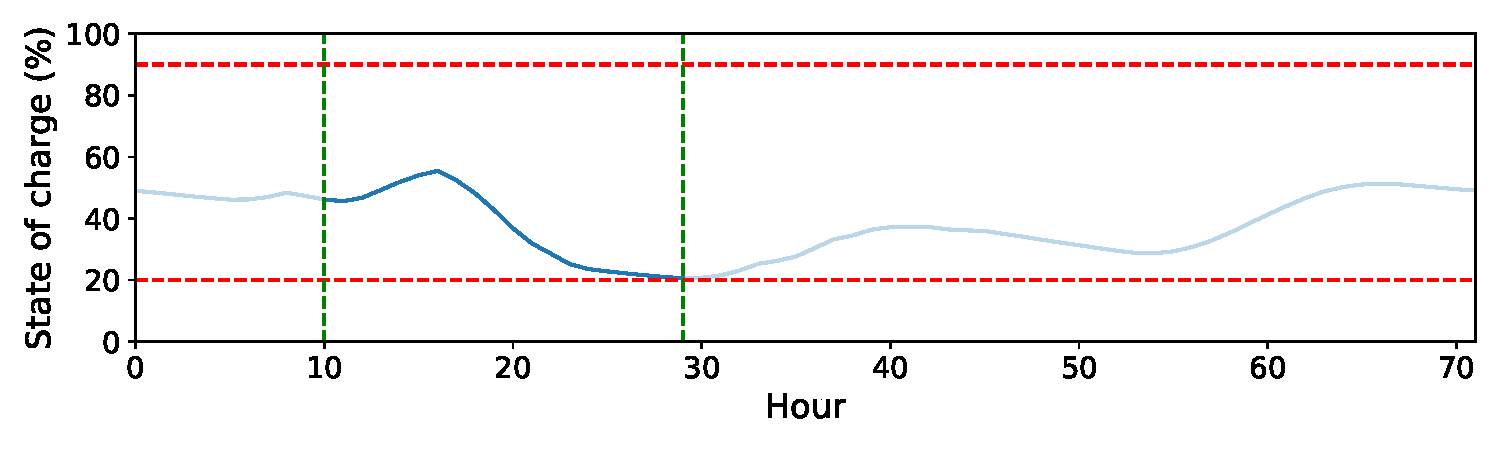
\includegraphics[scale=0.34]{Images/Heuristics/idle_machines.pdf}
    \caption{Verification of possible energy to save. In this example, the actual step is at hour 10. In this step, it needs to verify how much energy is possible to save from future steps. So, it verifies the idle servers from hour 10 to hour 29, because at hour 30 the state of charge is equal to 20\%. It can change the usage from hour 10 to hour 30 freely. Taking energy from after hour 30 could violate the lower threshold since we will use more energy from the batteries.}
    \label{fig:idle_machines_verification}
\end{figure}

These verifications do not increase the complexity. Verification 1 goes through the plan with limited size (e.g., in our three-day time window, we have a plan with 864 time steps). Verification 2-a is done together with verification 1. Verification 2-b is faster than the others since it can process fewer steps and it can stop when $E_{poss} >= \sum Ed_t^{'} - Ed_t$. Verification 3-c is just to apply the modifications. It recalculates the state of charge to maintain the SoC updated for the next jobs to schedule. So, if a job puts a future state of charge close to the lower threshold, the next job takes it into account. Continuing in algorithm \ref{alg:algo_scheduling_heuristic}, if the tests pass, then it starts the job (line 7). When it finds a job that can not be placed now, it starts to backfill (lines 9-17). Then, it finds the first moment to run this job (named priority job) in the future (line 9). So, it re-sorts the queue using $P_{B}$ (line 10), placing the other jobs in the servers (lines 11-16) without delaying the (future) priority job execution (line 13). Line 13 does the same verification as line 6.

As mentioned before, EASY backfilling sorts the jobs by $P_{R}$ and $P_{B}$. Our implementation starts with $P_{R}$ using Bounded Slowdown:
\begin{equation}
    bsld_j = \max(\frac{w_j + p_j}{\max(p_j, \tau)}, 1)
\end{equation}

Where:
\begin{itemize}
    \item \(bsld_j\): Bounded Slowdown of job \(j\);
    \item \(p_j\): Job \(j\) execution time (we consider the walltime here);
    \item \(w_j\): Job \(j\) waiting time;
    \item \(\tau\): Constant to avoid smaller jobs from reaching very high Bounded Slowdown (fixed in 10 seconds).
\end{itemize}

Bounded Slowdown estimates the ratio between the total time that a job stays in the system and its actual processing time. This order helps to let a job wait proportionately to its size. For $P_{B}$, \emph{\systemName} sorts the jobs by the smallest sizes first (walltime multiplied by the number of resources needed). This order helps in the backfill process since sometimes the "holes" in the scheduling demand very small jobs. Also, these jobs are less likely to demand more energy from future time steps (so, \emph{\systemName} lets the energy to the priority ones). Figure \ref{fig:estimated_state_of_charge} highlights a dangerous area. In this area, \emph{\systemName} changes $P_{R}$ to also use the smallest sizes first. These are not good moments to start big jobs, even if they are waiting too long in the queue. Small jobs demand less energy and are more likely to finish.

\subsection{Power compensation}
\label{sec:model_compensations}

After describing the scheduling algorithm, this section explains the heuristic to compensate for power fluctuations. While the scheduling algorithm runs for every job arrival, end, or server state modification, the power compensation algorithm will execute at every new time step. Since the scheduling algorithm modifies future time steps (it places the jobs in servers that are already on) and verifies the violations, we do not need to run the power compensations for every placement. Also, changing the server state too much between on and off can degrade it faster and takes time to power on/off. So, we defined that the state and speed stay constant inside each time step. 

The main objective of this part of the heuristic is to finish the time window with the state of charge as close as possible to the planned. Renewable sources can produce more or less than predicted. Also, the power usage can vary due to server idleness or scheduling modifications. So, at each time step, \emph{\systemName} calculates the state of charge for all future time steps using Equation \ref{equ:battery_state_of_charge}. Then, it calculates the energy difference $E_{diff}$ between the target and the estimated SoC at the end of the time window. For example, if the target level is 50\% and the estimated SoC is 51\%, $E_{diff}$ is 1\%. So, we need to reintroduce 1\% of the battery. On the other hand, if the estimated last SoC is 49\%, $E_{diff}$ is -1\%. So, we need to reduce the usage by 1\%. Therefore, it needs to reintroduce/remove the energy $E_{diff}$ before the end of the time window.

When the compensation is positive ($E_{diff}>0$), we can increase the speed of the servers or run more jobs. First, \emph{\systemName} uses the $E_{diff}$ to speed up the running jobs. It increases the speed from the actual time step to the time step that the job finishes. This helps in avoiding jobs to reach their walltime. After that, if there is still energy, it verifies if there are jobs in the waiting queue. If so, it turns on some servers to run these jobs. If there is not or it turned all the servers needed to run jobs, it lets the remaining energy in the battery. This is a conservative approach. \emph{\systemName} could be aggressive, using the remaining energy to turn on machines in the future. However, we prefer to finish with more energy in the batteries than expend this energy not wisely.

In the negative compensation ($E_{diff}<0$), \emph{\systemName} considers the estimated SoCs from Figure \ref{fig:estimated_state_of_charge}. First, it finds the time step with the higher number of predictions below 20\% or the last time step if there are no predictions below 20\% (let's name it the violation time step). The idea is to reduce the usage before the violation, reducing the violation probability. Then, \emph{\systemName} reduces servers speed in the following order (stopping when it is enough):
\begin{enumerate}
    \item Impacts idle servers from the violation time step to the actual time step (it goes through the time steps backward);
    \item Impacts idle servers from the violation time step to the last time step (it goes through the time steps forward);
    \item Impacts running servers from the violation time step to the last time step (it goes through the time steps forward);
    \item Impacts running servers from the violation time step to the actual time step (it goes through the time steps backward);
\end{enumerate}

\emph{\systemName} focuses first on idle servers because impacting not idle servers can increase the number of killed jobs. Killing jobs increases wasted energy. So, \emph{\systemName} searches for idle servers in both ways (violation time step $\rightarrow$ actual time step and violation time step $\rightarrow$ last time step). If reducing the usage from idle servers is not sufficient, we start to impact running servers (steps 3 and 4). Our idea is to impact them as far as possible from the actual step, but considering the violation step. The real total job execution time is uncertain (e.g., they could finish earlier than predicted). If we change the order (step 4 before step 3), the chance of really impacting the job is higher since it will reduce the energy from the violation step to the actual step. Doing step 3 before, we expect that the job finishes before these changes, while impacting the steps around the violation step. 

\section{Results Evaluation}

\section{Conclusion}